\vspace{-0.3cm}
\section{评测}
\vspace{-0.2cm}

我们将 \sys 与多种最先进方法和系统进行了广泛比较。结果表明：
\begin{enumerate}[label=(\arabic*),leftmargin=0.5cm,noitemsep,topsep=0pt]
\item 在 LLM 推理中，\sys 相比 T10 和 Ladder 获得了数量级的加速（第~\ref{sec:eval:e2e} 节）；
\item \sys 的 \gemm 和 \gemv 在性能与强扩展性上都优于最先进方法（第~\ref{sec:eval:meshgemm} 节）；
\item \sys 基于移位的 KV cache 管理把 token 容量提高了 $360$--$385\times$ 以上（第~\ref{sec:eval:kvcache} 节）；
\item 与 A100 GPU 集群上 SGLang 的最佳性能相比，Cerebras WSE-2 上的 \sys 取得 $10$--$20\times$ 端到端加速；与单块 A100 GPU 相比，加速约为 $30$--$40\times$。\sys 的能效也高出约 $2.5\times$（第~\ref{sec:eval:e2e}、\ref{sec:eval:gpu} 节）。
\end{enumerate}

\mypar{实验设置}
我们在一台配备 Cerebras WSE-2 的服务器上评测 \sys。WSE-2 拥有 850,000 个核心，每个核心都带有最高工作频率为 1.1GHz 的计算引擎（CE）。每个时钟周期可以从 SRAM 取入两个 32-bit 操作数，执行一次乘加运算，再把结果写回 SRAM。每个核心还有一个 fabric router，可在单个时钟周期内向邻近核心发送或从其接收 32-bit 消息。此外，每个核心包含 48KB SRAM，全芯片聚合 SRAM 容量为 40GB~\cite{wse}。

我们把 \sys 与两种 DNN 编译器进行比较：（i）T10~\cite{t10}，面向核心间互连和分布式片上内存 AI 加速器的最先进编译器；（ii）Ladder~\cite{ladder}，面向共享内存架构的最先进编译器。对于 T10，我们在 WSE-2 上实现该系统，并把每个核心视为由交叉开关互连的分布式内存系统的一部分，尽管实际拓扑是网格。T10 把数据映射到核心 ID，并按需从本地 SRAM 取入数据。对于 Ladder，我们把芯片上由网格互连的分布式内存架构视作统一内存，因此访问数据需要在 NoC 上执行集合通信。

GPU 对比实验使用 NVIDIA A100；为保证公平，它与 WSE-2 均采用 7nm 工艺。实验最多使用跨两个节点的 16 块 GPU（$2\times8$ 配置）。单节点内的 8 块 A100 通过 NVLink 互连，节点间通信使用高性能 InfiniBand（IB）网络。GPU 实验采用性能最高的 LLM 推理系统之一 SGLang~\cite{sglang}。

\mypar{评测指标} 为评估不同硬件上 LLM 推理系统的单请求最大吞吐性能，我们定义每请求吞吐量（Throughput per Request，TPR）这一关键指标。TPR 由更常用的每输出 token 时间（TPOT）推导而来：$\text{TPR}=\frac{1}{\text{TPOT}}$。

\mypar{LLM 模型}
评测覆盖了不同规模与架构的多种代表性 LLM。LLaMA3-8B 和 LLaMA2-13B 是广泛使用的开源 LLM；其中 LLaMA3 使用分组查询注意力而非多头注意力，以减少 KV cache 用量。对于 LLaMA2-13B，我们移除了模型的 4K 上下文长度限制，以评估系统在不同输入、输出长度下的性能。此外，受张量并行约束，模型的注意力头数必须能被所用 GPU 数整除，因此我们没有在 16-GPU 集群上开展 LLaMA2 的多 GPU 实验。CodeLLaMA-34B 是面向编程任务的专用 LLM，QWen2-72B 则是另一种以高模型质量著称的流行 LLM。

\vspace{-0.2cm}
\subsection{LLM 推理}\label{sec:eval:e2e}

我们首先报告 \sys 与 WSE-2 上 T10、Ladder 以及 A100 GPU 集群上 SGLang 的端到端性能比较；随后把执行拆分为预填充和解码阶段，以进一步分析性能并提供更深入的认识。

\begin{table}[t]
  \centering
  \resizebox{\linewidth}{!}{
    \begin{tabular}{l|cc|cccc}
\hline
\multicolumn{1}{c|}{\multirow{2}{*}{模型}} & \multicolumn{2}{c|}{\multirow{2}{*}{设备}} & \multicolumn{4}{c}{输入/输出序列长度} \\ \cline{4-7}
\multicolumn{1}{c|}{} & \multicolumn{2}{c|}{} & \multicolumn{1}{c|}{2048/128} & \multicolumn{1}{c|}{4096/128} & \multicolumn{1}{c|}{2048/2048} & 4096/4096 \\ \hline
\multirow{6}{*}{LLaMA3-8B} & \multicolumn{1}{c|}{\multirow{3}{*}{WSE-2}} & \sys & \multicolumn{1}{c|}{764.4} & \multicolumn{1}{c|}{604.4} & \multicolumn{1}{c|}{2370.3} & 2459.0 \\
 & \multicolumn{1}{c|}{} & T10 & \multicolumn{1}{c|}{4.6} & \multicolumn{1}{c|}{4.5} & \multicolumn{1}{c|}{58.3} & 94.6 \\
 & \multicolumn{1}{c|}{} & Ladder & \multicolumn{1}{c|}{1.2} & \multicolumn{1}{c|}{1.1} & \multicolumn{1}{c|}{7.4} & 8.7 \\ \cline{2-7}
 & \multicolumn{1}{c|}{\multirow{3}{*}{\begin{tabular}[c]{@{}c@{}}A100 GPU\\（SGLang）\end{tabular}}} & 1 & \multicolumn{1}{c|}{34.8} & \multicolumn{1}{c|}{31.1} & \multicolumn{1}{c|}{36.5} & 78.4 \\
 & \multicolumn{1}{c|}{} & 8 & \multicolumn{1}{c|}{117.2} & \multicolumn{1}{c|}{109.0} & \multicolumn{1}{c|}{128.4} & 256.1 \\
 & \multicolumn{1}{c|}{} & $2\times8$ & \multicolumn{1}{c|}{73.7} & \multicolumn{1}{c|}{70.2} & \multicolumn{1}{c|}{79.3} & 162.5 \\ \hline
\multirow{5}{*}{LLaMA2-13B} & \multicolumn{1}{c|}{\multirow{3}{*}{WSE-2}} & \sys & \multicolumn{1}{c|}{473.9} & \multicolumn{1}{c|}{414} & \multicolumn{1}{c|}{1690.3} & 1826.0 \\
 & \multicolumn{1}{c|}{} & T10 & \multicolumn{1}{c|}{2.6} & \multicolumn{1}{c|}{2.5} & \multicolumn{1}{c|}{35.0} & 58.3 \\
 & \multicolumn{1}{c|}{} & Ladder & \multicolumn{1}{c|}{0.7} & \multicolumn{1}{c|}{0.7} & \multicolumn{1}{c|}{4.9} & 6.1 \\ \cline{2-7}
 & \multicolumn{1}{c|}{\multirow{2}{*}{\begin{tabular}[c]{@{}c@{}}A100 GPU\\（SGLang）\tablefootnote{\label{missing_16GPU}受模型架构和张量并行约束，没有 $2\times8$ GPU 结果。}\end{tabular}}} & 1 & \multicolumn{1}{c|}{20.4} & \multicolumn{1}{c|}{17.1} & \multicolumn{1}{c|}{21.1} & 47.9 \\
 & \multicolumn{1}{c|}{} & 8 & \multicolumn{1}{c|}{79.6} & \multicolumn{1}{c|}{70.5} & \multicolumn{1}{c|}{86.9} & 172.4 \\ \hline
\end{tabular}%
    }
  \caption{端到端 LLM 推理的 TPR}
  \label{tab:e2e_table}
\end{table}

\mypar{端到端吞吐量} 表~\ref{tab:e2e_table} 给出了不同输入、输出序列长度下，LLaMA3-8B 和 LLaMA2-13B 在 WSE-2 与 A100 上的推理 TPR。这里，端到端吞吐量等于解码阶段生成的 token 总数除以预填充和解码两个阶段的总时间。\sys 针对每个模型使用经过优化、能获得最佳性能的核心配置：LLaMA3-8B 的预填充使用 $660\times660$ 个核心，解码使用 $360\times360$ 个核心；LLaMA2-13B 的预填充使用 $750\times750$ 个核心，解码使用 $375\times375$ 个核心。由于单颗 WSE-2 的内存容量不足，表中未包含 CodeLLaMA-34B 和 QWen2-72B。

与 T10 相比，对于 4096 或 2048 输入上下文、输出 128 个 token 的短序列生成任务，\sys 平均加速 $160\times$，最高 $180\times$；对于输入上下文分别为 4096、2048 token，输出长度分别为 4096、2048 token 的较长任务，平均加速 $36\times$，最高 $48\times$。T10 的 compute-shift 模型虽然考虑了 PLMR 设备的内存约束（M）和路由资源限制（R），却没有考虑核心由网格 NoC 互连这一事实，因此既无法处理不同跳数带来的差异（L），也无法扩展到数百万核心（P）。这说明，超大规模 NUMA 架构需要新的系统设计。

与 Ladder 相比，对于上述输出 128 个 token 的短序列生成任务，\sys 平均加速 $625\times$，最高 $677\times$；对于上述较长序列生成任务，平均加速 $312\times$，最高 $342\times$。原因在于 Ladder 面向共享内存架构设计，没有考虑 PLMR 设备特性，因而无法把 LLM 划分到数百万核心（P），会产生代价高昂的长距离 NoC 通信（L），也无法处理本地内存约束（M）和有限路由资源（R）。

\begin{table}[t]
\centering
\resizebox{\linewidth}{!}{
\begin{tabular}{c|c|ccclccc}
\cline{1-5} \cline{7-9}
\multirow{2}{*}{模型} & \multirow{2}{*}{方法} & \multicolumn{3}{c}{WSE-2 核心} & & \multicolumn{3}{c}{A100 GPU 数（SGLang）} \\ \cline{3-5} \cline{7-9}
 & & \multicolumn{1}{c|}{$480\times480$} & \multicolumn{1}{c|}{$600\times600$} & $720\times720$ & & \multicolumn{1}{c|}{1} & \multicolumn{1}{c|}{8} & $2\times8$ \\ \cline{1-5} \cline{7-9}
\multirow{3}{*}{LLaMA3-8B} & \sys & \multicolumn{1}{c|}{20320.6} & \multicolumn{1}{c|}{25037.2} & 27686.5 & & \multicolumn{1}{c|}{\multirow{3}{*}{13988.3}} & \multicolumn{1}{c|}{\multirow{3}{*}{17361.6}} & \multirow{3}{*}{13994.2} \\
 & T10 & \multicolumn{1}{c|}{175.0} & \multicolumn{1}{c|}{156.6} & 132.8 & & \multicolumn{1}{c|}{} & \multicolumn{1}{c|}{} & \\
 & Ladder & \multicolumn{1}{c|}{61.8} & \multicolumn{1}{c|}{42.3} & 31.3 & & \multicolumn{1}{c|}{} & \multicolumn{1}{c|}{} & \\ \cline{1-5} \cline{7-9}
\multirow{3}{*}{LLaMA2-13B} & \sys & \multicolumn{1}{c|}{13685.1} & \multicolumn{1}{c|}{16854.2} & 17498.3 & & \multicolumn{1}{c|}{\multirow{3}{*}{7805.1}} & \multicolumn{1}{c|}{\multirow{3}{*}{12287.1}} & \multirow{3}{*}{/\textsuperscript{\ref{missing_16GPU}}} \\
 & T10 & \multicolumn{1}{c|}{121.3} & \multicolumn{1}{c|}{100.6} & 81.3 & & \multicolumn{1}{c|}{} & \multicolumn{1}{c|}{} & \\
 & Ladder & \multicolumn{1}{c|}{47.3} & \multicolumn{1}{c|}{33.1} & 24.2 & & \multicolumn{1}{c|}{} & \multicolumn{1}{c|}{} & \\ \cline{1-5} \cline{7-9}
\multirow{3}{*}{CodeLLaMA-34B} & \sys & \multicolumn{1}{c|}{5471.4} & \multicolumn{1}{c|}{7540.1} & 8526 & & \multicolumn{1}{c|}{\multirow{3}{*}{5382.5}} & \multicolumn{1}{c|}{\multirow{3}{*}{7155.5}} & \multirow{3}{*}{6409.2} \\
 & T10 & \multicolumn{1}{c|}{49.1} & \multicolumn{1}{c|}{46.8} & 41.2 & & \multicolumn{1}{c|}{} & \multicolumn{1}{c|}{} & \\
 & Ladder & \multicolumn{1}{c|}{30.1} & \multicolumn{1}{c|}{23.1} & 17.7 & & \multicolumn{1}{c|}{} & \multicolumn{1}{c|}{} & \\ \cline{1-5} \cline{7-9}
\multirow{3}{*}{QWen2-72B} & \sys & \multicolumn{1}{c|}{2785.2} & \multicolumn{1}{c|}{3775.5} & 4421.6 & & \multicolumn{1}{c|}{\multirow{3}{*}{1677.3}} & \multicolumn{1}{c|}{\multirow{3}{*}{3803.8}} & \multirow{3}{*}{3750.5} \\
 & T10 & \multicolumn{1}{c|}{24.9} & \multicolumn{1}{c|}{23.5} & 21.5 & & \multicolumn{1}{c|}{} & \multicolumn{1}{c|}{} & \\
 & Ladder & \multicolumn{1}{c|}{16.8} & \multicolumn{1}{c|}{12.8} & 10.1 & & \multicolumn{1}{c|}{} & \multicolumn{1}{c|}{} & \\ \cline{1-5} \cline{7-9}
\end{tabular}%
}
  \caption{预填充阶段的每请求吞吐量（TPR）}
  \vspace{-0.2cm}
\label{tab:prefill_throughput}
\end{table}

\mypar{预填充吞吐量} 表~\ref{tab:prefill_throughput} 给出了输入序列长度为 4096、核心配置从 $480\times480$ 到 $720\times720$ 时的预填充性能。CodeLLaMA-34B 与 QWen2-72B 超出 WSE-2 和单块 A100 的内存容量，因此我们评测其中若干层，并依据各层结构均匀这一特点按比例缩放结果。

\sys 通过有效处理全部 PLMR 属性，获得了显著加速：相比 T10 平均约 $160\times$、最高 $178\times$；相比 Ladder 约 $270$--$450\times$。如第~\ref{sec:motivation} 节所述，GEMM 是主要瓶颈，而 \gemm 显著提升了 \sys 的预填充性能；第~\ref{sec:eval:meshgemm} 节将对此作详细分析。

此外，\sys 在所有模型上都能随核心数增加而提升吞吐量。例如，当核心规模从 $480\times480$ 扩大到 $720\times720$ 时，QWen2-72B 提升 $1.6\times$，LLaMA3-8B 提升 $1.4\times$。相反，T10 和 Ladder 无法有效扩展，增加核心后吞吐量甚至会下降。主要原因是 T10 与 Ladder 没有考虑高度非均匀分布式内存的空间局部性（L），因而可能频繁跨核心远距离读取数据，增加通信开销。

\begin{table}[t]
  \centering
  \resizebox{\linewidth}{!}{
    \begin{tabular}{c|c|ccclccc}
\cline{1-5} \cline{7-9}
\multirow{2}{*}{模型} & \multirow{2}{*}{方法} & \multicolumn{3}{c}{WSE-2 核心} & & \multicolumn{3}{c}{A100 GPU 数（SGLang）} \\ \cline{3-5} \cline{7-9}
 & & \multicolumn{1}{c|}{$420\times420$} & \multicolumn{1}{c|}{$540\times540$} & $660\times660$ & & \multicolumn{1}{c|}{1} & \multicolumn{1}{c|}{8} & $2\times8$ \\ \cline{1-5} \cline{7-9}
\multirow{3}{*}{LLaMA3-8B} & \sys & \multicolumn{1}{c|}{2699.9} & \multicolumn{1}{c|}{2501.5} & 2243.3 & & \multicolumn{1}{c|}{\multirow{3}{*}{78.9}} & \multicolumn{1}{c|}{\multirow{3}{*}{260.4}} & \multirow{3}{*}{164.6} \\
 & T10 & \multicolumn{1}{c|}{418.3} & \multicolumn{1}{c|}{339.4} & 265.1 & & \multicolumn{1}{c|}{} & \multicolumn{1}{c|}{} & \\
 & Ladder & \multicolumn{1}{c|}{14.6} & \multicolumn{1}{c|}{13.1} & 11.4 & & \multicolumn{1}{c|}{} & \multicolumn{1}{c|}{} & \\ \cline{1-5} \cline{7-9}
\multirow{3}{*}{LLaMA2-13B} & \sys & \multicolumn{1}{c|}{2039.2} & \multicolumn{1}{c|}{1899.4} & 1739.8 & & \multicolumn{1}{c|}{\multirow{3}{*}{48.7}} & \multicolumn{1}{c|}{\multirow{3}{*}{175.8}} & \multirow{3}{*}{/\textsuperscript{\ref{missing_16GPU}}} \\
 & T10 & \multicolumn{1}{c|}{341.8} & \multicolumn{1}{c|}{270.8} & 233.7 & & \multicolumn{1}{c|}{} & \multicolumn{1}{c|}{} & \\
 & Ladder & \multicolumn{1}{c|}{11.0} & \multicolumn{1}{c|}{9.9} & 9.0 & & \multicolumn{1}{c|}{} & \multicolumn{1}{c|}{} & \\ \cline{1-5} \cline{7-9}
\multirow{3}{*}{CodeLLaMA-34B} & \sys & \multicolumn{1}{c|}{1450.8} & \multicolumn{1}{c|}{1407.7} & 1359.2 & & \multicolumn{1}{c|}{\multirow{3}{*}{26.1}} & \multicolumn{1}{c|}{\multirow{3}{*}{100.4}} & \multirow{3}{*}{84.5} \\
 & T10 & \multicolumn{1}{c|}{278.2} & \multicolumn{1}{c|}{222.4} & 193.1 & & \multicolumn{1}{c|}{} & \multicolumn{1}{c|}{} & \\
 & Ladder & \multicolumn{1}{c|}{6.1} & \multicolumn{1}{c|}{6.2} & 5.8 & & \multicolumn{1}{c|}{} & \multicolumn{1}{c|}{} & \\ \cline{1-5} \cline{7-9}
\multirow{3}{*}{QWen2-72B} & \sys & \multicolumn{1}{c|}{839.7} & \multicolumn{1}{c|}{824.3} & 787.1 & & \multicolumn{1}{c|}{\multirow{3}{*}{10.6}} & \multicolumn{1}{c|}{\multirow{3}{*}{51.2}} & \multirow{3}{*}{48.7} \\
 & T10 & \multicolumn{1}{c|}{168.5} & \multicolumn{1}{c|}{133.0} & 114.6 & & \multicolumn{1}{c|}{} & \multicolumn{1}{c|}{} & \\
 & Ladder & \multicolumn{1}{c|}{3.2} & \multicolumn{1}{c|}{3.3} & 3.4 & & \multicolumn{1}{c|}{} & \multicolumn{1}{c|}{} & \\ \cline{1-5} \cline{7-9}
\end{tabular}%
    }
  \caption{解码阶段的每请求吞吐量（TPR）}
  \vspace{-0.2cm}
\label{tab:decode_throughput}
\end{table}

\mypar{解码吞吐量} 表~\ref{tab:decode_throughput} 给出了核心配置从 $420\times420$ 到 $660\times660$ 时的解码吞吐量。对于 CodeLLaMA-34B 和 QWen2-72B 在 WSE-2 与单块 A100 上的解码基准，我们同样评测若干层并按比例缩放结果。

通过处理全部 PLMR 属性，\sys 相比 T10 平均加速 $5.7\times$、最高 $6.5\times$；相比 Ladder 平均加速 $217\times$、最高 $260\times$。

\sys 在预填充阶段相对 T10 加速 $160\times$，但在解码阶段只加速约 $6.5\times$；相比之下，它在预填充和解码阶段都能稳定保持相对 Ladder 的 $200$--$500\times$ 优势。主要原因是，预填充涉及 dist-GEMM 计算，要求每个数据元素按照固定顺序穿过同一行或同一列上的核心；解码中的 dist-GEMV allreduce 则只要求遍历同一行或同一列的核心，并不强制严格访问顺序。T10 的 compute-shift 范式虽然没有考虑网格 NoC 上核心的空间局部性，但仍考虑了分布式内存，所以当内存（通信）访问与顺序无关时仍可获得性能收益。Ladder 则完全针对共享内存架构设计，无论是否要求内存访问顺序，都会产生严重通信开销。

\mypar{与 SGLang 比较} 如表~\ref{tab:e2e_table}、\ref{tab:prefill_throughput} 和 \ref{tab:decode_throughput} 所示，从 8B 到 72B 的多种模型上，\sys 在预填充、解码和端到端性能方面都明显优于 SGLang 与 A100 GPU 集群。第~\ref{sec:eval:gpu} 节将进一步讨论与 GPU 的比较。

值得注意的是，与 SGLang 相比，T10 和 Ladder 未能利用 WSE-2 强大的硬件能力。例如，在预填充任务以及 Ladder 的解码任务中，它们的性能甚至低于单块 A100 上的 SGLang。这表明，在晶圆级芯片上设计高性能系统与算法必须仔细考虑 PLMR 模型；否则，芯片的海量计算潜力不仅无法得到利用，大规模网格 NoC 造成的高度非均匀分布式内存还可能使性能下降。

\vspace{-0.2cm}
\subsection{\gemm}\label{sec:eval:meshgemm}
\vspace{-0.2cm}

\begin{figure}
    \centering
    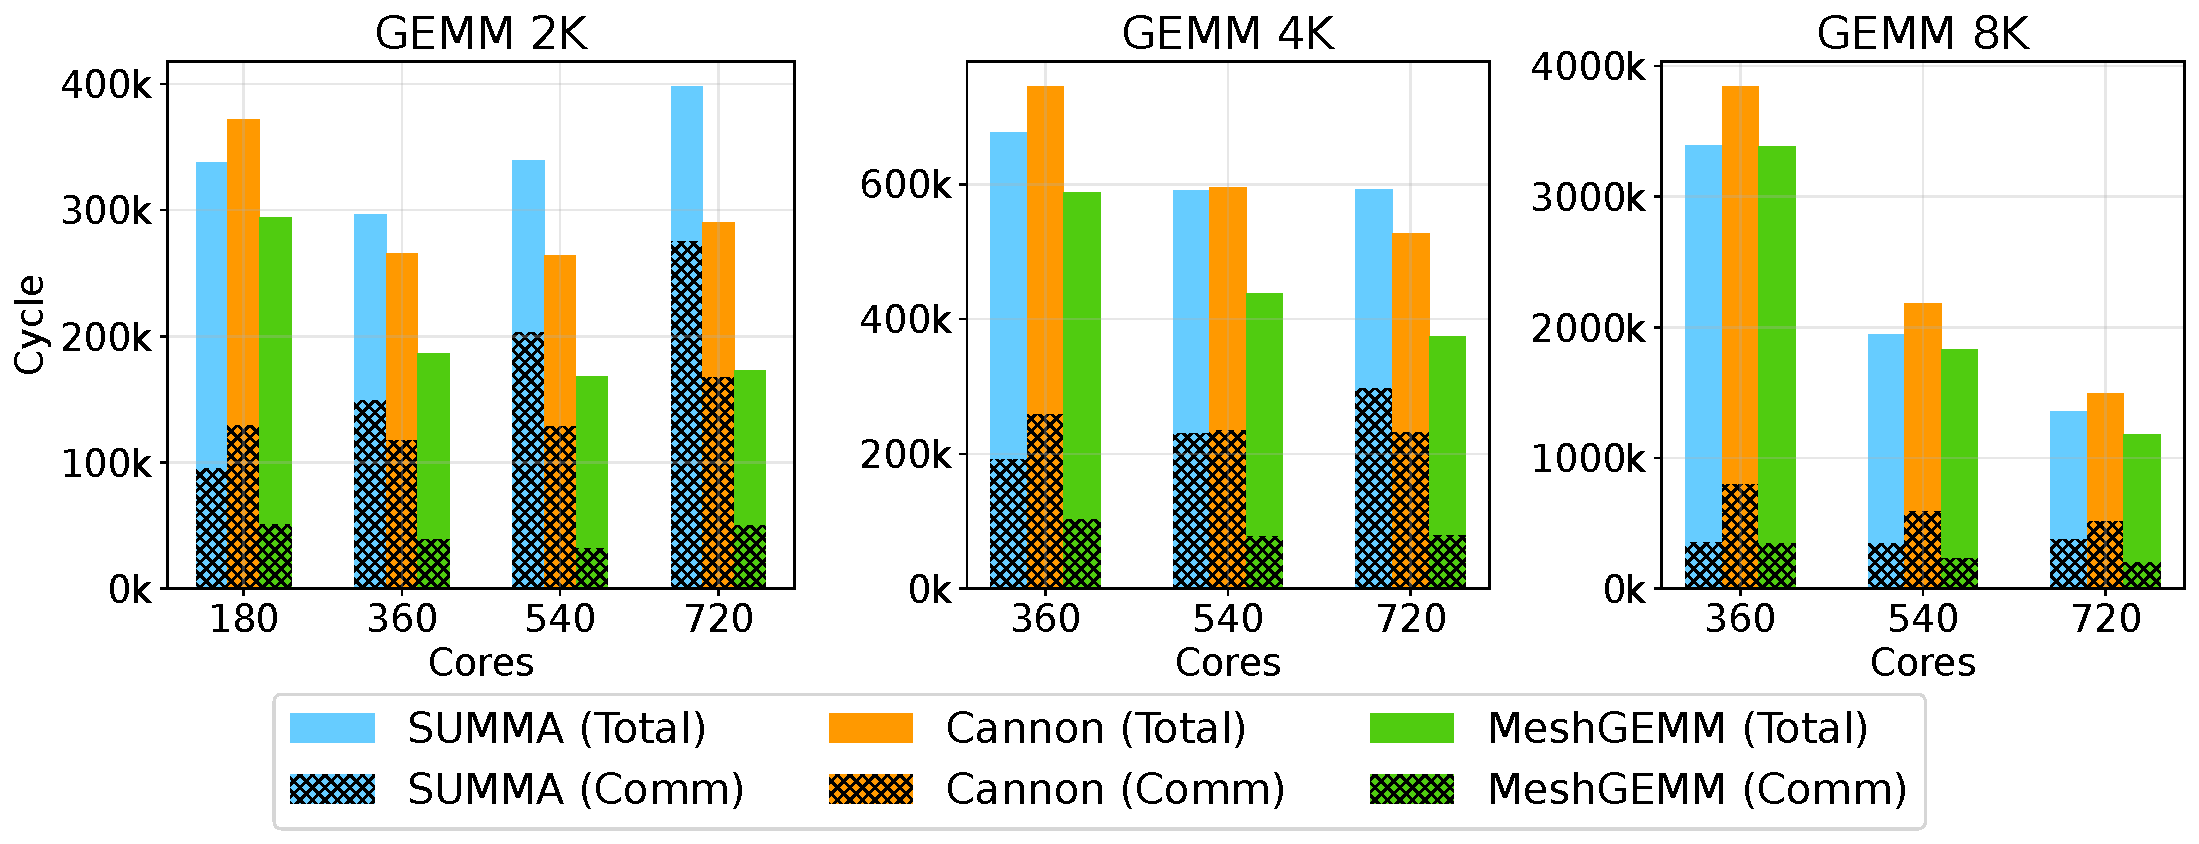
\includegraphics[width=1\linewidth]{imgs/gemm_micro_benchmark_combined.pdf}
    \caption{\gemm 与 SUMMA、Cannon 的比较}
    \vspace{-0.5cm}
    \label{fig:eval:meshgemm}
\end{figure}

我们在 WSE-2 上，针对不同核心规模与矩阵大小，将 \gemm 与 Cannon~\cite{cannon}、SUMMA~\cite{summa} 进行比较。

\mypar{扩展核心数}
图~\ref{fig:eval:meshgemm} 表明，对于不同大小的矩阵，\gemm 在增加核心数时都能取得低于 SUMMA 和 Cannon 的延迟。相比 SUMMA 的流水线广播与 Cannon 的头到尾传输，\gemm 的交错传输可以尽量降低每一步的通信开销，并在大规模细粒度并行执行时尽可能重叠通信与计算。它展现出更强的可扩展性，即使接近硬件极限也能保持 70\% 以上的计算效率。SUMMA 与 Cannon 的扩展性则较差：使用 $720\times720$ 个核心时，计算效率降至 50\% 以下，主要原因是其通信开销随并行规模增长。

此外，增加核心数并不总能提高性能，小矩阵 GEMM 尤其如此。例如，对于 GEMM 2K，当核心规模从 $360\times360$ 扩大到 $720\times720$ 时，SUMMA 和 Cannon 的端到端延迟不降反升。原因是，核心数超过某个阈值后，单核计算成本只会次线性下降（受函数调用、逻辑检查等固定开销影响），同时通信开销却线性增长，如图~\ref{fig:eval:meshgemm} 中阴影区域所示，最终使总体性能恶化。相比之下，\gemm 在 $720\times720$ 个核心上仅略微增加通信开销，并保持稳定的端到端延迟。这是因为交错通信把每一步的通信成本限制为与核心数无关的常数（所有 dist-GEMM 算法的总通信开销仍会因步数增加而增长）。因此，即使在大规模细粒度并行下——每个核心只负责少量数据——\gemm 也能更好地重叠通信与计算。

\mypar{扩展矩阵大小} 我们还使用更大的矩阵评测 \gemm，使 GEMM 成为计算强度更高的运算。在大规模下，通信成本的重要性虽然降低，\gemm 仍保持可扩展性，并以较大优势优于 SUMMA 和 Cannon，把总周期减少约 17\%。

图~\ref{fig:eval:meshgemm} 中一个有趣现象是：对于 GEMM 8K，通信周期会随核心数增加而减少。这是因为处理大量数据时，通信受带宽而非延迟限制。增加核心数不仅提高聚合算力、降低计算开销，还增加聚合带宽，从而降低总体通信成本。

\vspace{-0.2cm}
\subsection{\gemv}
\vspace{-0.2cm}

我们在不同核心规模和矩阵形状下，将 \gemv 与 Cerebras 的默认 GEMV 实现（流水线 allreduce）进行比较。

\begin{figure}
    \centering
    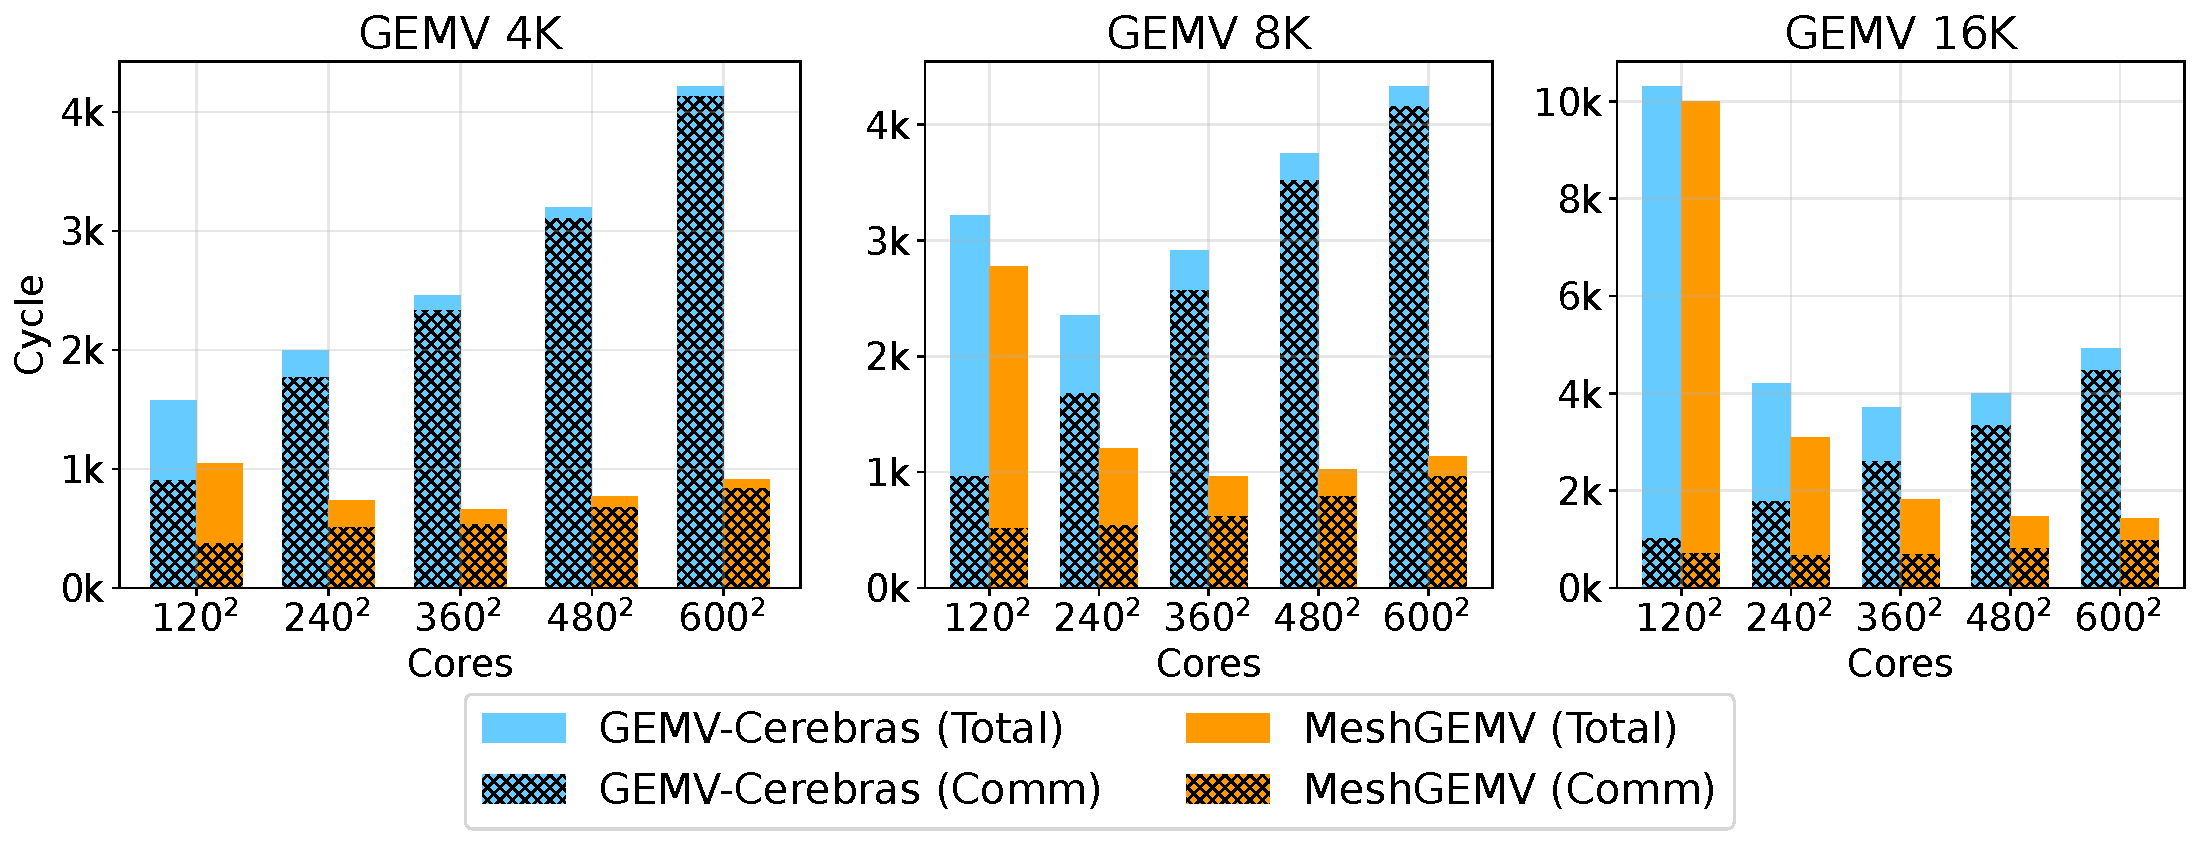
\includegraphics[width=1\linewidth]{imgs/gemv_micro_benchmark_combined.pdf}
    \caption{\gemv 与 Cerebras GEMV 的比较}
    \vspace{-0.3cm}
    \label{fig:eval:meshgemv}
\end{figure}

\mypar{通信延迟瓶颈} 图~\ref{fig:eval:meshgemv} 表明，通信已成为 WSE-2 上 dist-GEMV 的主要瓶颈；当并行规模相对单核计算量很大时，通信开销甚至可占总开销的 90\% 以上。不过，与 Cerebras 基线 GEMV 相比，\gemv 显著降低了通信开销，端到端性能提高约 $4.6\times$。原因是大规模 dist-GEMV 需要长距离 allreduce 通信，而 \gemv 使用 K 树 allreduce，最大化 allreduce 过程的并行度，从而尽量降低关键路径上的通信与计算成本。

\mypar{扩展核心数和矩阵大小} 我们还用更大的矩阵评测 \gemv。与 2K 相比，基线在 GEMV 8K 和 16K 上的端到端开销呈现先降后升的趋势。最初的下降来自核心数增加：更高的聚合算力与带宽降低了计算和通信成本；但核心数继续增长后，allreduce 通信延迟最终超过计算与带宽，成为主要瓶颈。\gemv 的拐点出现得更晚，这意味着对于相同数据规模，随核心数增长，其通信开销的增速远低于基线，表现出更好的可扩展性。这使片上映射策略更灵活，例如可以用更多核心存储额外 LLM 参数，以满足内存限制（M），同时不引入显著额外开销。

\vspace{-0.3cm}
\subsection{基于移位的 KV cache 管理}\label{sec:eval:kvcache}
\vspace{-0.2cm}

\begin{table}[t]
  \centering
  \resizebox{0.8\linewidth}{!}{
    \begin{tabular}{l|c|c}
    \hline
    模型 & LLaMA3-8B & LLaMA2-13B \\
    \hline
    基于拼接（PagedAttention） & 382 & 16 \\
    \hline
    基于移位（\sys） & 137548 & 6168 \\
    \hline
    \end{tabular}%
    }
  \caption{最大解码输出长度}
  \label{tab:eval:kvcache}
\end{table}

我们还将基于移位的 KV cache 管理与 PagedAttention 中基于拼接的方案进行比较。实验使用 LLaMA3-8B 与 LLaMA2-13B，并采用第~\ref{sec:eval:e2e} 节端到端推理评测的相同设置来测量 KV cache 容量。表~\ref{tab:eval:kvcache} 表明，对于 LLaMA3-8B 和 LLaMA2-13B，\sys 基于移位的 KV cache 管理分别比拼接方案多支持 $360\times$ 和 $385\times$ 的 token。该提升来自均衡的核心利用率，以及移位方案对数据倾斜问题的消除。

\vspace{-0.2cm}
\subsection{与 GPU 比较}\label{sec:eval:gpu}
\vspace{-0.2cm}

\begin{table}[t]
  \centering
  \resizebox{\linewidth}{!}{
    \begin{tabular}{c|ccc|ccc}
\hline
GEMV & \multicolumn{3}{c|}{[1,16K]$\times$[16K,16K]} & \multicolumn{3}{c}{[1,32K]$\times$[32K,32K]} \\ \hline
\multirow{2}{*}{\begin{tabular}[c]{@{}c@{}}SGLang（A100）的 TP\\时间（ms）\end{tabular}} & 1 GPU & 8 GPU & $2\times8$ GPU & 1 GPU & 8 GPU & $2\times8$ GPU \\ \cline{2-7}
 & 0.336 & 0.253 & 0.340 & 1.231 & 0.341 & 0.339 \\ \hline
\begin{tabular}[c]{@{}c@{}}\gemv（WSE-2）\\时间（ms）\end{tabular} & & 0.0012 & & & 0.00203 & \\ \hline
A100/WSE-2 能耗比 & \textbf{7.47} & \textbf{44.97} & \textbf{120.88} & \textbf{16.17} & \textbf{35.83} & \textbf{71.25} \\ \hline
\end{tabular}%
    }
  \caption{比较 \gemv（WSE-2）与 SGLang（A100）张量并行的 GEMV 延迟和能耗。}
  \vspace{-0.3cm}
  \label{tab:mv_gpu}
\end{table}

我们使用 Cerebras WSE-2 和 NVIDIA A100，将 \sys 与 GPU 上最先进的 LLM 推理系统进行比较。若要与 H100 公平比较，则需要使用同为 5nm 工艺的 WSE-3，但我们无法获得该设备。

\mypar{GEMV} 我们将 \gemv 与遵循 SGLang~\cite{sglang} 多 GPU 张量并行的 GEMV 并行策略进行比较；每块 GPU 上的计算使用 cuBLAS 加速。如表~\ref{tab:mv_gpu} 所示，针对不同矩阵大小，\gemv 比单块 A100 GPU 快 $280$--$606\times$，展示了晶圆级设备提供巨大内存带宽的优势。其能效也高出 $7.5$--$16\times$，体现了晶圆内连接（连接片上内存）相对 GPU 中基于 PCB 的连接（连接片外 HBM）的优势。

多 GPU 分布式 GEMV 的可扩展性有限：单块 A100 的每 FLOP 能效最高；从一块扩展到八块 GPU 时，性能仅提高 $1.32\times$，扩展到十六块后反而下降。这种低效率源于内存密集性，以及 NVLink 和 IB 上的通信开销。相比之下，\gemv 利用 WSE-2 的低延迟 NoC，在数十万个核心上扩展；与 GPU 集群的最佳结果相比，峰值性能高出 $166$--$210\times$，能效高出 $45$--$70\times$。此外，在两台机器共 16 块 GPU 上，16K 与 32K GEMV 的性能相近，主要是因为跨两节点分布式 GEMV 的通信开销主导了计算。

尽管有这些优势，\gemv 仍未达到理论上的 $7{,}000\times$ 提升。性能剖析发现有三个原因：（i）仍处于第二代的 WSE-2 核心无法完全重叠内存访问与计算；（ii）边缘核心利用不足；（iii）尽管 \gemv 已有效缓解，NoC 长距离通信开销依然存在。我们预计，随着晶圆级加速器成熟，这些差距会继续缩小。

\begin{table}[t]
  \centering
  \resizebox{\linewidth}{!}{
    \begin{tabular}{c|ccc|cc}
\hline
预填充（4K 上下文） & \multicolumn{3}{c|}{LLaMA3-8B} & \multicolumn{2}{c}{LLaMA2-13B} \\ \hline
\multirow{2}{*}{SGLang（A100）TPR} & 1 GPU & 8 GPU & $2\times8$ GPU & 1 GPU & 8 GPU \\ \cline{2-6}
 & 13988 & 17361 & 13994 & 7805 & 12287 \\ \hline
\sys WSE-2 TPR & & 27686 & & \multicolumn{2}{c}{17498} \\ \hline
A100/WSE-2 能耗比 & \textbf{0.05} & \textbf{0.34} & \textbf{0.84} & \textbf{0.06} & \textbf{0.30} \\ \hline
\end{tabular}%
    }
  \caption{比较 \sys（WSE-2）与 SGLang（A100）的预填充吞吐量和能耗。}
  \vspace{-0.3cm}
  \label{tab:llmoc_gpu_prefill}
\end{table}

\begin{table}[t]
  \centering
  \resizebox{\linewidth}{!}{
    \begin{tabular}{c|ccc|cc}
\hline
解码（4K 上下文） & \multicolumn{3}{c|}{LLaMA3-8B} & \multicolumn{2}{c}{LLaMA2-13B} \\ \hline
\multirow{2}{*}{SGLang（A100）TPR} & 1 GPU & 8 GPU & $2\times8$ GPU & 1 GPU & 8 GPU \\ \cline{2-6}
 & 78 & 260 & 164 & 48 & 175 \\ \hline
\sys WSE-2 TPR & & 2700 & & \multicolumn{2}{c}{2039} \\ \hline
A100/WSE-2 能耗比 & \textbf{0.92} & \textbf{2.22} & \textbf{7.02} & \textbf{1.13} & \textbf{2.49} \\ \hline
\end{tabular}%
    }
  \caption{比较 \sys（WSE-2）与 SGLang（A100）的解码吞吐量和能耗。}
  \vspace{-0.3cm}
  \label{tab:llmoc_gpu_decode}
\end{table}

\mypar{LLM 推理} GPU 集群可达到的最大 TPR 显著低于 WSE-2。我们把 \sys 与多 A100 GPU 集群上的 SGLang 进行比较后发现，在多种输入/输出长度以及从 8B 到 72B 的模型规模上，\sys 的 TPR 高出 $6$--$20\times$；输出越长、模型越大，差距越明显（表~\ref{tab:e2e_table}）。如表~\ref{tab:llmoc_gpu_prefill} 和表~\ref{tab:llmoc_gpu_decode} 所示，SGLang 从 1 块扩展到 8 块 GPU 时，预填充仅加速 $1.2$--$1.6\times$，解码仅加速 $3.3$--$3.6\times$，远低于理想的线性扩展。受节点间通信瓶颈影响，扩展到 16 块 GPU 后性能进一步下降。因此，稠密模型的峰值 TPR 通常出现在单个 8-GPU 节点内，而 \sys 相比这一配置仍最高快 $20\times$。对于要求较高单请求吞吐量的场景，晶圆级加速器的能力显著强于传统 xPU 系统。

能效方面，虽然一颗 WSE-2 的面积约为 A100 的 $47\times$，功耗和成本约为 A100 的 $37\times$，但由于 GPU 的解码扩展不是线性的，\sys 相比 SGLang 的最佳多 GPU 结果仍有 $2$--$2.5\times$ 能效优势。对于测试时扩展等长输出场景，这一优势尤其重要，因为服务成本是关键因素。不过，与单独的 GEMV 相比，\sys 的解码能效优势有所缩小，原因包括：（i）WSE-2 核心的本地 SRAM 只有 48KB，妨碍高效张量并行，并迫使系统采用流水线并行，导致利用率最高降低 $5\times$；（ii）面向 GPU 优化的 LLaMA 模型具有较窄的层，限制了 WSE-2 上的层放置并进一步降低利用率。
